\chapter{不确定性、埃伦费斯特定理与经典极限}

\section{线性哈密顿量中的未了结之处}

模型
\begin{equation}
H=cP
\label{eq:l10-linear-hamiltonian}
\end{equation}
之所以有用，是因为它的波包在平移时不改变形状。它也带来一个严重的警告。动量可以为正也可以为负，因此同一个公式对一个平面波赋予正能量，而对另一个平面波赋予负能量：
\begin{equation}
\psi_p(x)=e^{ipx/\hbar},
\qquad
E(p)=cp.
\end{equation}
如果任意多个物理粒子都能占据负能量态，那么真空就不会是最低能量状态。它可以产生正能量量子，同时把补偿性的负能量沉积到新粒子中，从而保持总能量不变，却使真空能量无下界地降低。

\begin{classroomqa}
\audiencequestion{为什么负能量分支不只是对能量零点的一种奇怪选择？}
\lecturerresponse{对每个能量作共同的加性平移是无害的。无下界的谱则不同。如果总能布居越来越低能量的态，而正能量粒子带走差额，那就不存在稳定的基态。稳定性要求相对于真空有下界。}
\end{classroomqa}

\begin{figure}[htbp]
\centering
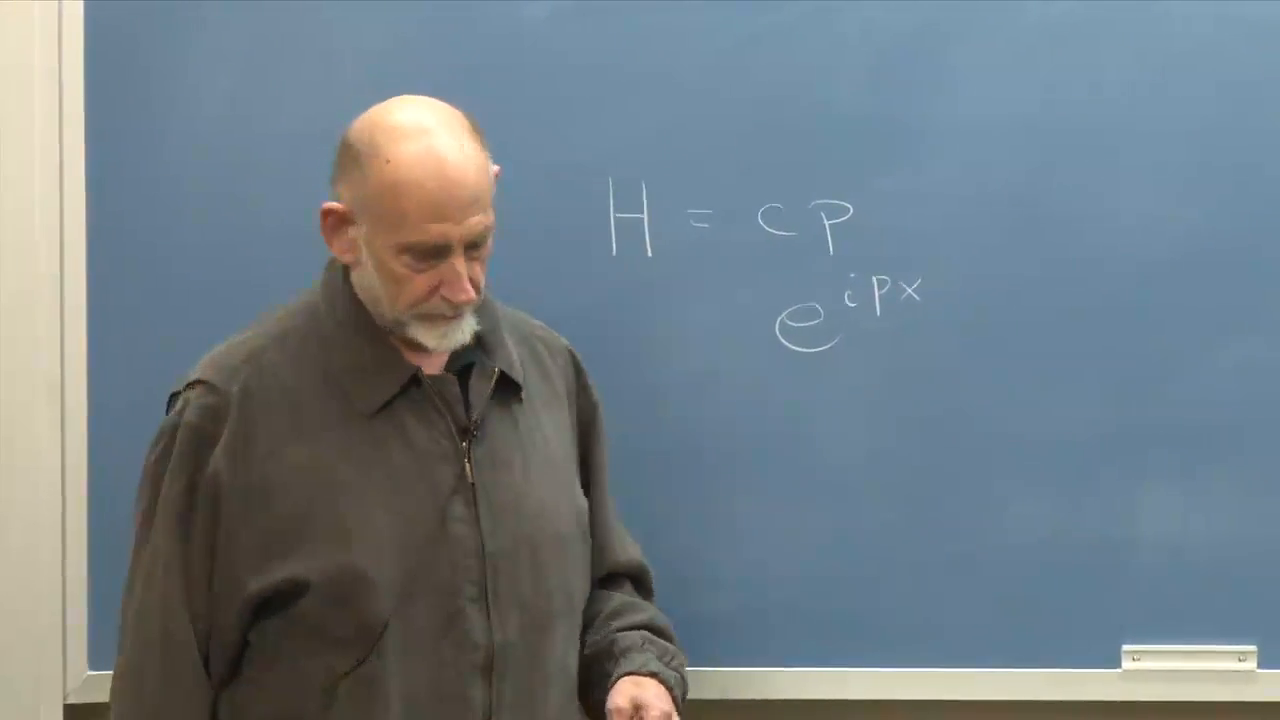
\includegraphics[width=0.88\textwidth]{lecture_10_figure_01.png}
\caption{线性哈密顿量及其平面波本征函数在\(p<0\)时暴露出负能量分支。}
\lectureframe{00:04:35}
\end{figure}

狄拉克历史上的回答对费米子有效。费米子服从不相容原理：没有两个全同费米子能占据同一个单粒子态。想象把每一个负能量态都填满。一旦它们全被占据，不相容原理就阻止另一个费米子落入该区域。被填满集合中的一个空位表现为一个反粒子。

这一论证并不能拯救负能量玻色子。任意多个玻色子都可以占据一个态，因此一个负能量玻色子模式可以被无限制地布居。旧的填满海图像最好被视为通向反粒子的历史途径；现代量子场论组织粒子与反粒子时，并不把物理真空当作字面意义上可观测负能量电子的海。这里所需的要点更窄：这个玩具哈密顿量并不是一个完整的稳定粒子理论。

作为对以固定速率运动的费米子的一维漫画式描述，该模型暗示了中微子问题，而狄拉克的想法正与此相关。它不能充当光子理论：光子是玻色子，不相容原理无法填满并阻挡它们的负能量态。

\begin{classroomqa}
\audiencequestion{为什么不相容原理能稳定费米子构造，却不能稳定玻色子构造？}
\lecturerresponse{一个费米子态可以被填满一次，然后被阻挡。一个玻色子态没有这样的占据上限，因此一个负能量玻色子模式仍会让能量无下界地降低。}
\end{classroomqa}

\paragraph{课程目前所处的位置。}
本学季已经建立了量子力学的许多基础，并讨论了若干刻意简单的系统，但应用极少。特别是，它甚至还没有讲到谐振子。这一遗漏标志着一个边界，而不是终点：接下来是相对论和场论，之后必须再次拾起量子力学，以研究谐振子以及建立在它之上的其他结构。早先关于纠缠的讨论所引发的持续兴趣，也说明了为什么走基础路线是值得的。

有了这一视角，未了结之处就闭合了。主要事务是波函数、不确定性，以及量子演化与经典力学之间的关系。目标不是尽可能一般的演化方程，而是最初由Schr\"odinger写下的那个特殊的位形空间方程。

\section{波函数与完全对易坐标}

对于直线上的一个粒子，位形空间波函数是
\begin{equation}
\psi(x)=\braket{x}{\psi},
\end{equation}
即在\(x\)附近找到该粒子的振幅。动量空间波函数是
\begin{equation}
\widetilde{\psi}(p)=\braket{p}{\psi}.
\end{equation}
它们在不同的基中描述同一个抽象态，并通过傅里叶变换相联系：
\begin{align}
\psi(x)
&=
\int_{-\infty}^{\infty}
\frac{dp}{\sqrt{2\pi\hbar}}\,
\widetilde{\psi}(p)e^{ipx/\hbar},
\label{eq:l10-fourier-forward}\\
\widetilde{\psi}(p)
&=
\int_{-\infty}^{\infty}
\frac{dx}{\sqrt{2\pi\hbar}}\,
\psi(x)e^{-ipx/\hbar}.
\label{eq:l10-fourier-inverse}
\end{align}

\begin{figure}[htbp]
\centering
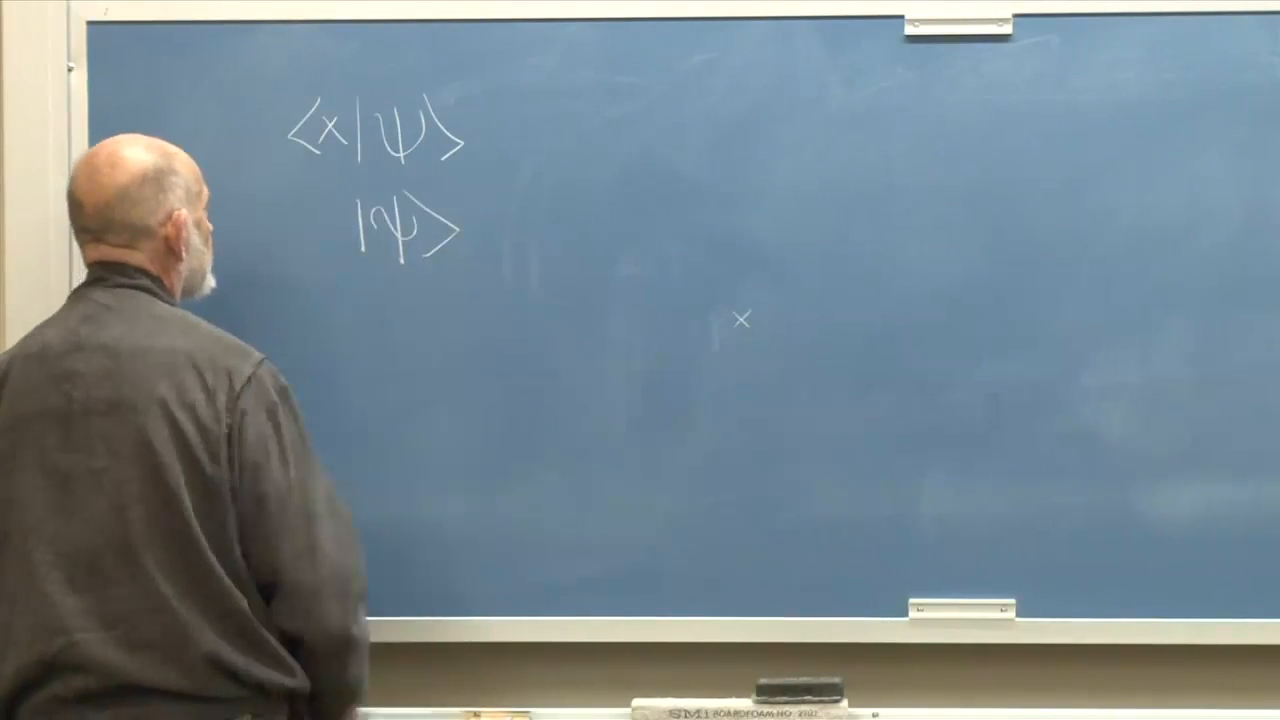
\includegraphics[width=0.88\textwidth]{lecture_10_figure_02.png}
\caption{位置波函数和动量波函数是同一个态在两个不同连续基上的投影。}
\lectureframe{00:09:05}
\end{figure}

在二维空间中，\(X\)和\(Y\)对易，因此可以用两个坐标共同标记一个共同本征基，而波函数变为\(\psi(x,y)\)。这种对易并不是仅由抽象公理强制的；它是关于普通空间的、经验上成功的量子描述的一部分。对于三维空间中的\(N\)个粒子，
\begin{equation}
\psi(\mathbf{x}_1,\ldots,\mathbf{x}_N)
\end{equation}
是位形空间上的函数，而不是独立附着于每个粒子的另一个三维波。因此，一个宏观系统可能需要数量极其巨大的坐标。

\begin{classroomqa}
\audiencequestion{不同空间坐标的对易性是否自动由量子力学得出？}
\lecturerresponse{不。抽象框架允许许多可观测量代数。不同的笛卡尔位置分量对易这一事实，是关于普通空间中粒子量子力学的一个经验性结构事实。}
\end{classroomqa}

人们可以对每个坐标作傅里叶变换，得到所有动量的波函数，也可以只变换选定的变量。混合表象是合法的，因为表象是基的选择，而不是物理状态的改变。

\section{不确定性度量的是什么}

不确定性原理最原始的形式直接来自傅里叶对。具有确定动量的态是模为常数的平面波，没有位置局域化。位置高度局域化的态需要许多动量分量。更一般地，使傅里叶对中的一个成员变窄会使另一个变宽。

\begin{figure}[htbp]
\centering
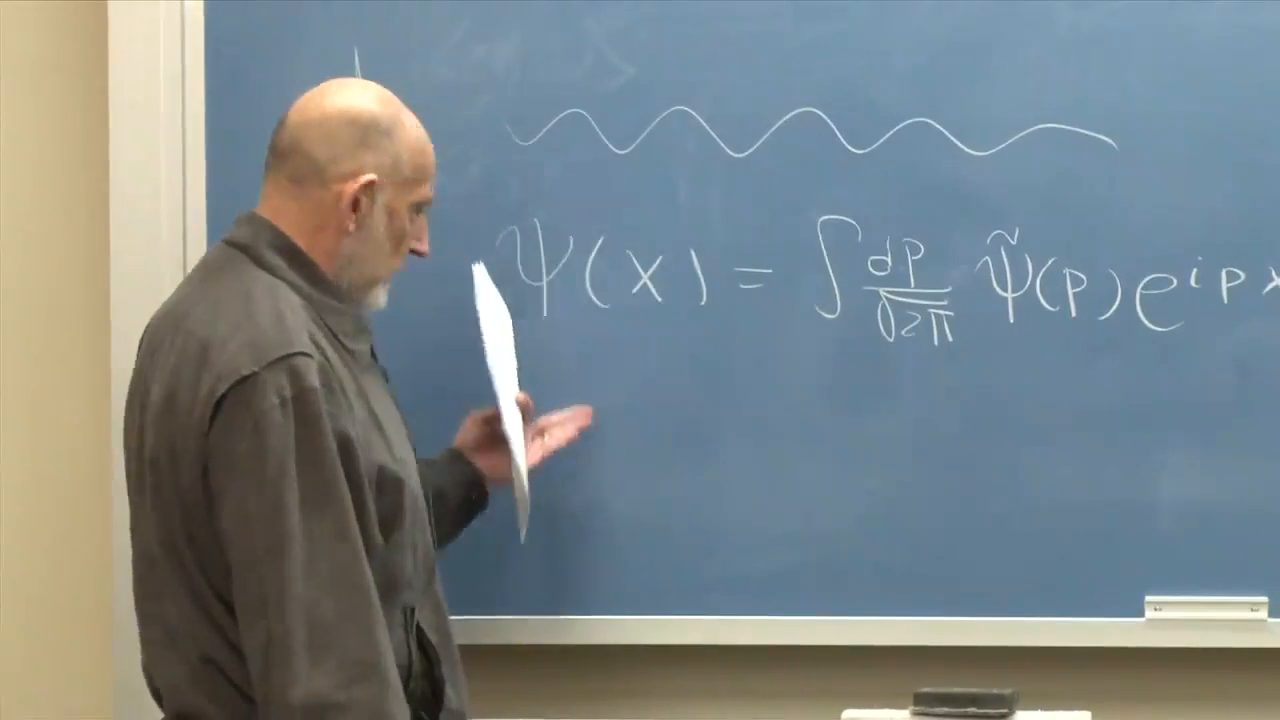
\includegraphics[width=0.88\textwidth]{lecture_10_figure_03.png}
\caption{局域化的位置分布要求在互易的动量表象中是平面波的宽叠加。}
\lectureframe{00:14:45}
\end{figure}

为了使这一陈述定量化，从一个一般的可观测量\(Q\)开始。它在归一化态中的期望值是
\begin{equation}
\expect{Q}=\bra{\psi}Q\ket{\psi}.
\end{equation}
方差是
\begin{equation}
(\Delta Q)^2
=
\expect{\bigl(Q-\expect{Q}\bigr)^2}
=
\expect{Q^2}-\expect{Q}^2.
\label{eq:l10-general-variance}
\end{equation}
不确定度\(\Delta Q\)是这个方差的正平方根。

对于位置，可以先平移原点使\(\expect{X}=0\)。于是
\begin{equation}
(\Delta x)^2
=
\expect{X^2}
=
\int_{-\infty}^{\infty}
dx\,|\psi(x)|^2x^2.
\label{eq:l10-position-variance}
\end{equation}
正贡献和负贡献在\(\expect{X}\)中相消，但在\(\expect{X^2}\)中相加。因此，更宽的概率分布具有更大的方差。

\begin{figure}[htbp]
\centering
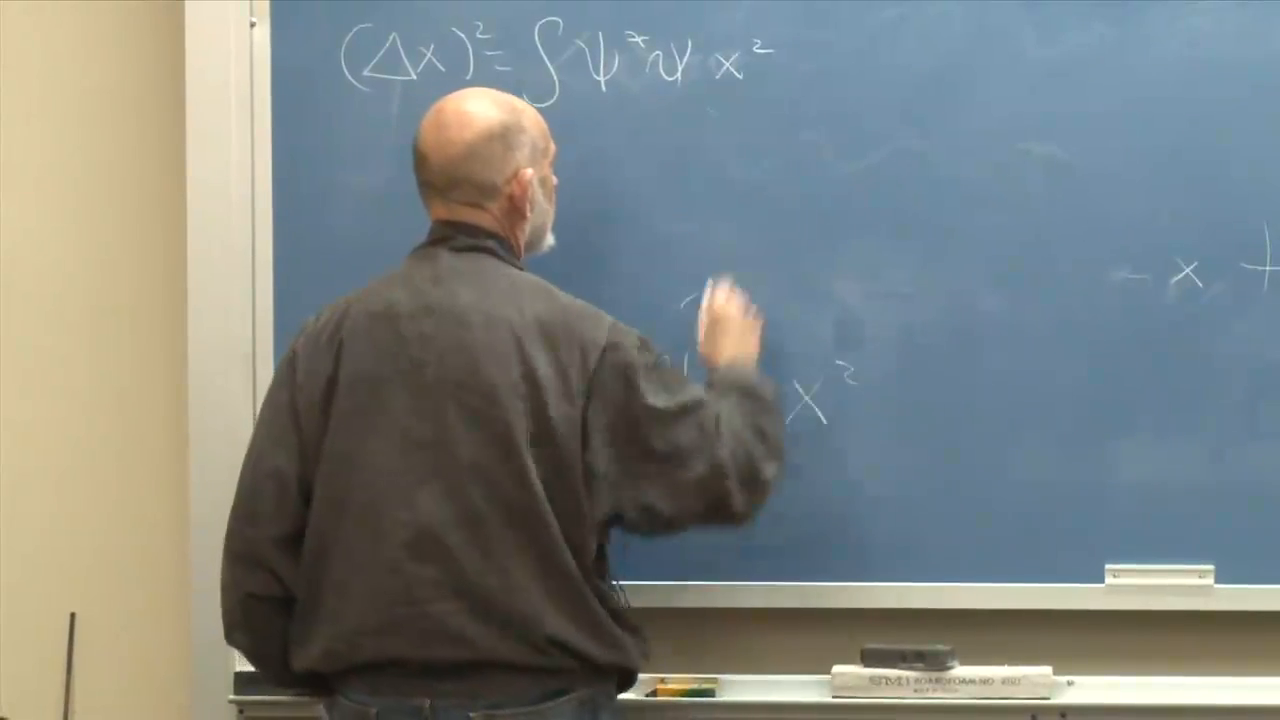
\includegraphics[width=0.88\textwidth]{lecture_10_figure_04.png}
\caption{将均值平移到零后，位置方差是\(x^2\)的概率加权积分。}
\lectureframe{00:20:50}
\end{figure}

\(\expect{X^2}\)与\(\expect{X}^2\)之间的区别至关重要。关于零对称的分布有\(\expect{X}=0\)，但除非它集中在原点，否则它仍然有\(\expect{X^2}>0\)。

动量方差可以直接在动量空间中定义：
\begin{equation}
(\Delta p)^2
=
\int_{-\infty}^{\infty}
dp\,|\widetilde{\psi}(p)|^2
\bigl(p-\expect{P}\bigr)^2.
\end{equation}
对于证明来说，在位置空间中处理更有用。将动量均值平移到零并使用
\begin{equation}
P=-i\hbar\frac{d}{dx},
\qquad
P^2=-\hbar^2\frac{d^2}{dx^2}.
\end{equation}
于是
\begin{equation}
(\Delta p)^2
=
\expect{P^2}
=
-\hbar^2
\int_{-\infty}^{\infty}
dx\,\psi^*(x)\frac{d^2\psi}{dx^2}.
\label{eq:l10-momentum-variance-second}
\end{equation}

\begin{classroomqa}
\audiencequestion{当一个方差的位形空间公式以负号开头时，它怎么可能是正的？}
\lecturerresponse{乘以该负号的积分是非正的。分部积分将一个导数转移到\(\psi^*\)上，引入第二个负号，并将结果变为一个绝对平方的积分。}
\end{classroomqa}

对于在无穷远处衰减足够快的波函数，
\begin{equation}
\int f\,g'\,dx
=
\left[fg\right]_{-\infty}^{\infty}
-
\int f'g\,dx,
\end{equation}
并且边界项消失。将其应用于式~\eqref{eq:l10-momentum-variance-second}一次，得到
\begin{equation}
(\Delta p)^2
=
\hbar^2
\int_{-\infty}^{\infty}
dx\,
\frac{d\psi^*}{dx}
\frac{d\psi}{dx}
=
\hbar^2
\int_{-\infty}^{\infty}
dx\,
\left|\frac{d\psi}{dx}\right|^2
\geq 0.
\label{eq:l10-momentum-variance-positive}
\end{equation}

\begin{figure}[htbp]
\centering
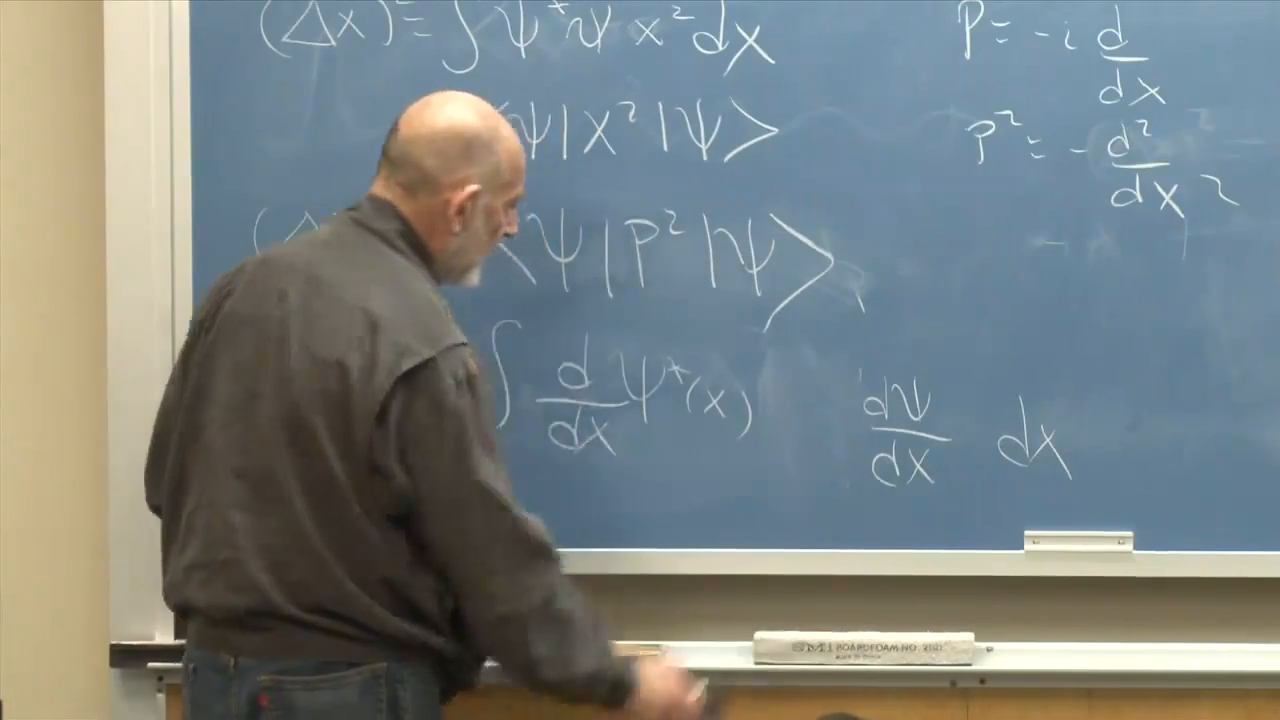
\includegraphics[width=0.88\textwidth]{lecture_10_figure_05.png}
\caption{分部积分将\(\expect{P^2}\)表面上为负的表达式转化为一个明显为正的范数。}
\lectureframe{00:27:35}
\end{figure}

\begin{classroomqa}
\audiencequestion{位置和动量的均值能否同时平移到零？}
\lecturerresponse{可以。平移波函数的自变量会移动\(\expect{X}\)，而将其乘以平面波相位会移动\(\expect{P}\)。这些操作改变均值而不改变相应的方差，因此证明中可以使用两个中心化变量。}
\end{classroomqa}

\section{不确定性下界}

所需的数学工具是柯西--施瓦茨不等式。本讲通过初等向量几何来引入它：两个向量的点积是它们长度乘以它们之间夹角的余弦，因此其大小不能超过它们长度的乘积。用希尔伯特空间记号表示，
\begin{equation}
\braket{A}{A}\braket{B}{B}
\geq
\left|\braket{A}{B}\right|^2.
\label{eq:l10-cauchy-schwarz}
\end{equation}
它在任意维度的实或复向量空间中都成立。

\begin{figure}[htbp]
\centering
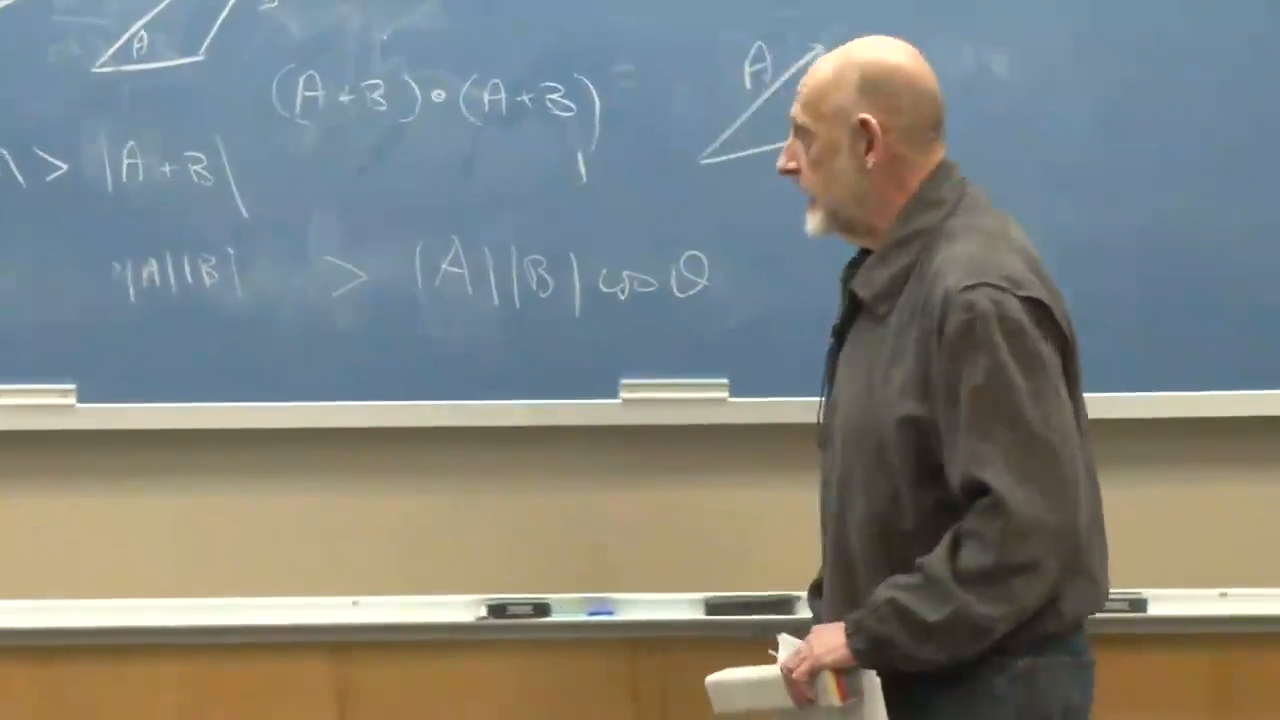
\includegraphics[width=0.88\textwidth]{lecture_10_figure_06.png}
\caption{几何向量不等式被改写为证明中使用的希尔伯特空间柯西--施瓦茨界。}
\lectureframe{00:35:35}
\end{figure}

\begin{classroomqa}
\audiencequestion{该不等式应当是严格的，还是等号可以成立？}
\lecturerresponse{它是一个大于或等于的关系。当两个希尔伯特空间向量线性相关时等号成立。该等号条件随后确定了最小不确定度波包。}
\end{classroomqa}

将两个变量都中心化，首先跟随简化的黑板证明，其中取\(\psi(x)\)为实数。定义
\begin{equation}
\ket{A}=X\ket{\psi},
\qquad
\ket{B}=P\ket{\psi}.
\label{eq:l10-auxiliary-vectors}
\end{equation}
它们的平方范数正是方差：
\begin{equation}
\braket{A}{A}=(\Delta x)^2,
\qquad
\braket{B}{B}=(\Delta p)^2.
\end{equation}

\begin{figure}[htbp]
\centering
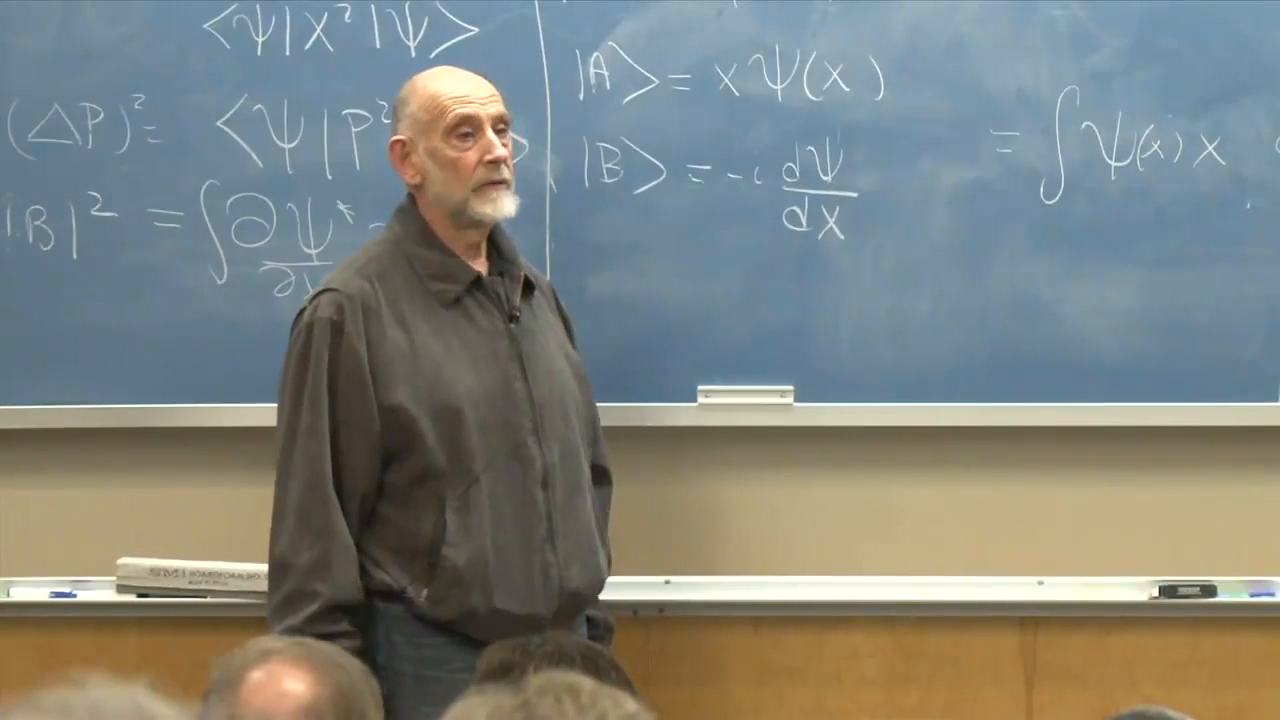
\includegraphics[width=0.88\textwidth]{lecture_10_figure_07.png}
\caption{辅助向量\(X\ket{\psi}\)和\(P\ket{\psi}\)将两个方差转化为希尔伯特空间范数。}
\lectureframe{00:44:40}
\end{figure}

剩下的内积是
\begin{align}
\braket{A}{B}
&=
\int_{-\infty}^{\infty}
dx\,
x\psi(x)
\left(-i\hbar\frac{d\psi}{dx}\right).
\end{align}
只有它的绝对值进入其中。由于\(\psi\)是实的，
\begin{equation}
\psi\frac{d\psi}{dx}
=
\frac{1}{2}\frac{d}{dx}\psi^2.
\end{equation}
因此，
\begin{align}
\left|\braket{A}{B}\right|
&=
\frac{\hbar}{2}
\left|
\int_{-\infty}^{\infty}
dx\,
x\frac{d}{dx}\psi^2
\right| \notag\\
&=
\frac{\hbar}{2}
\left|
-\int_{-\infty}^{\infty}
dx\,\psi^2
\right|
=
\frac{\hbar}{2},
\label{eq:l10-inner-product-half-hbar}
\end{align}
其中分部积分从\(\psi^2\)、\(d x/dx=1\)中去掉了导数，边界项消失，而归一化给出了最后一个等号。

将式~\eqref{eq:l10-inner-product-half-hbar}代入Cauchy--Schwarz不等式：
\begin{equation}
(\Delta x)^2(\Delta p)^2
\geq
\frac{\hbar^2}{4}.
\end{equation}
取正平方根得到
\begin{equation}
\boxed{
\Delta x\,\Delta p
\geq
\frac{\hbar}{2}
}.
\label{eq:l10-uncertainty-principle}
\end{equation}

\begin{figure}[htbp]
\centering
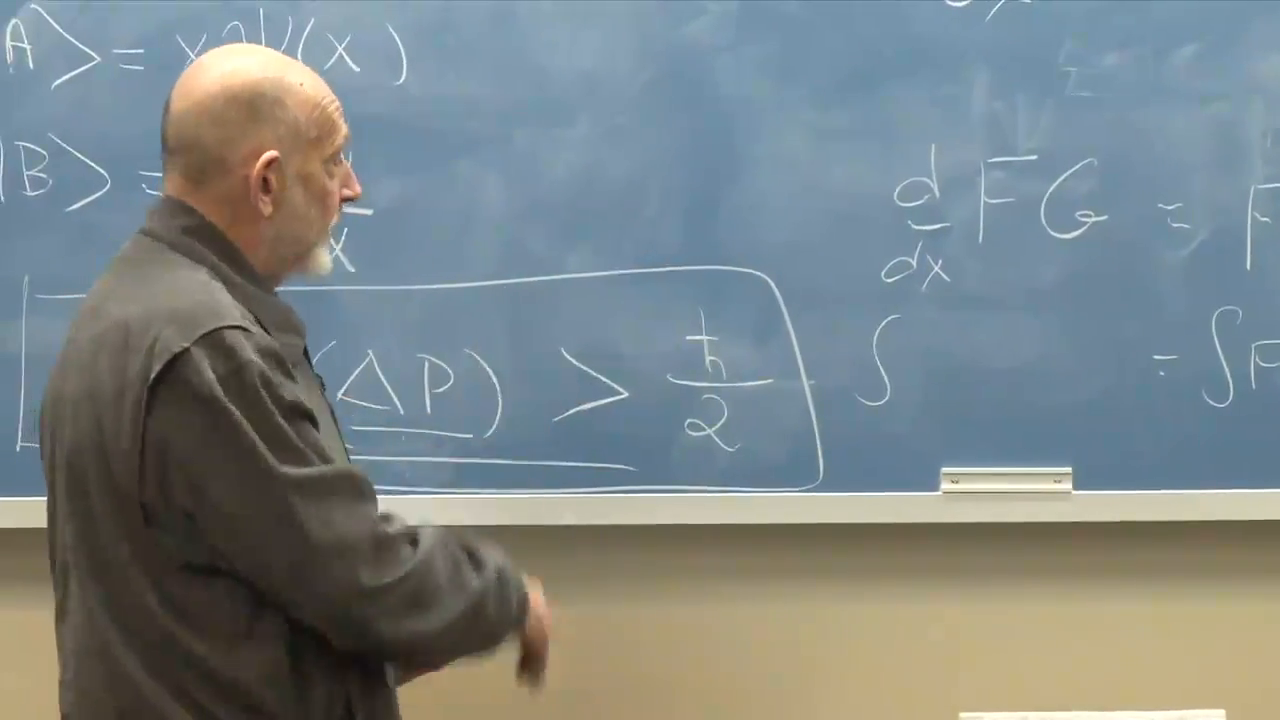
\includegraphics[width=0.88\textwidth]{lecture_10_figure_08.png}
\caption{分部积分步骤和归一化给出了尖锐的位置-动量不确定性下界。}
\lectureframe{00:50:55}
\end{figure}

对实\(\psi\)的限制只是黑板上的方便，而不是对定理的限制。对于一般的复态，取
\begin{equation}
\ket{A}=(X-\expect{X})\ket{\psi},
\qquad
\ket{B}=(P-\expect{P})\ket{\psi}.
\end{equation}
对易子确定了它们重叠部分的虚部：
\begin{equation}
\operatorname{Im}\braket{A}{B}
=
\frac{1}{2i}\expect{[X,P]}
=
\frac{\hbar}{2}.
\end{equation}
由于\(|\braket{A}{B}|\)至少与其虚部的模一样大，同样的界随之成立。

\begin{classroomqa}
\audiencequestion{在反复分部积分中，边界项究竟发生了什么？}
\lecturerresponse{对于这里所考虑的可归一化波包，出现在\(+\infty\)和\(-\infty\)处的乘积为零。在有限周期区间上，端点项相互抵消。必须选择算子的定义域，使这些陈述成立；否则形式上的操作就没有依据。}
\end{classroomqa}

\begin{classroomqa}
\audiencequestion{等号在物理上可以达到吗，还是下界仅仅是一个估计？}
\lecturerresponse{它是可以达到的。Cauchy--Schwarz不等式中的等号要求两个辅助矢量成比例。解出这个条件就得到高斯波包，也就是接下来要展开的最小不确定态。}
\end{classroomqa}

\section{其他傅里叶共轭对}

时间与能量之间的不确定性关系类似于位置与动量之间的关系。然而，它需要更加小心，因为在这里时间通常是一个演化参数，而不是由某个普适自伴算子表示的观测量。将态按能量本征矢量展开：
\begin{equation}
\ket{\psi(t)}
=
\int dE\,
\phi(E)e^{-iEt/\hbar}\ket{E}.
\label{eq:l10-time-energy-fourier}
\end{equation}
能量振幅与时间变化通过傅里叶关系相联系。窄的能量分布变化缓慢，不能形成时间上尖锐的脉冲；宽的能量分布则可以产生短的到达时间包络。

\begin{figure}[htbp]
\centering
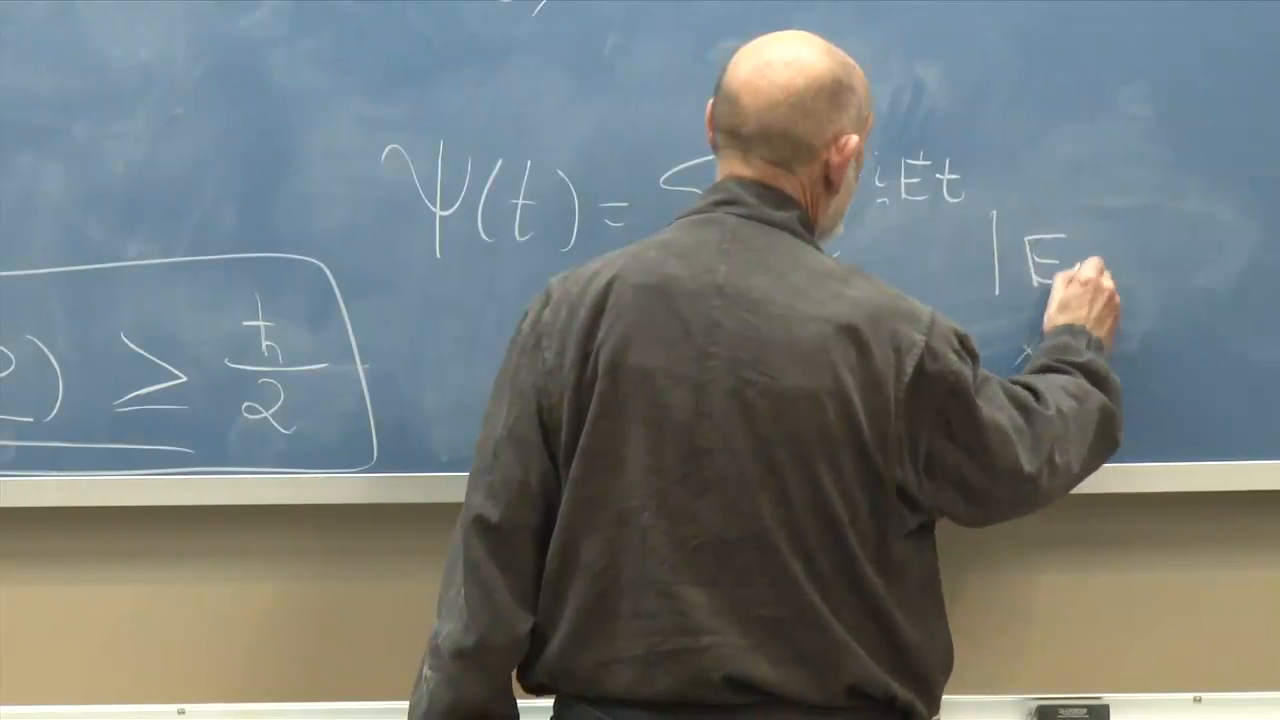
\includegraphics[width=0.88\textwidth]{lecture_10_figure_09.png}
\caption{时间依赖性由带有相位\(e^{-iEt/\hbar}\)的能量本征态组装而成，给出时间-能量关系的傅里叶基。}
\lectureframe{00:53:40}
\end{figure}

\begin{classroomqa}
\audiencequestion{同样的证明能直接适用于时间和能量吗？}
\lecturerresponse{倒易宽度的直觉可以，而一个经过的波包给出了有用的例子：短的到达时间窗口需要宽的能量分布。算子的陈述则更为微妙，因为时间进入这一表述的方式并不完全像\(X\)那样。}
\end{classroomqa}

角度和角动量构成旋转运动的另一对共轭量。局部地看，它们的傅里叶关系类似于位置和动量。整体地看，角度的周期性引入了额外的谨慎，因此这里的评述是一种类比，而不是完整的定理。

\begin{classroomqa}
\audiencequestion{位置-动量、时间-能量以及角度-角动量是孤立的例子吗？}
\lecturerresponse{不是。正则共轭变量反复作为傅里叶对出现。定义域和周期性的细节各不相同，但倒易局域化是共同的结构。}
\end{classroomqa}

\section{位置空间中的Schr\"odinger方程}

现在我们回到动力学。抽象定律是
\begin{equation}
i\hbar\frac{d}{dt}\ket{\psi(t)}
=
H\ket{\psi(t)}.
\label{eq:l10-abstract-schrodinger}
\end{equation}
对于质量为\(m\)、处于势\(V(X)\)中的粒子，取
\begin{equation}
H=\frac{P^2}{2m}+V(X).
\label{eq:l10-particle-hamiltonian}
\end{equation}
这引入了经典的动能加势能形式，然后检验其量子演化是否在适当的范围内再现经典运动。

\begin{figure}[htbp]
\centering
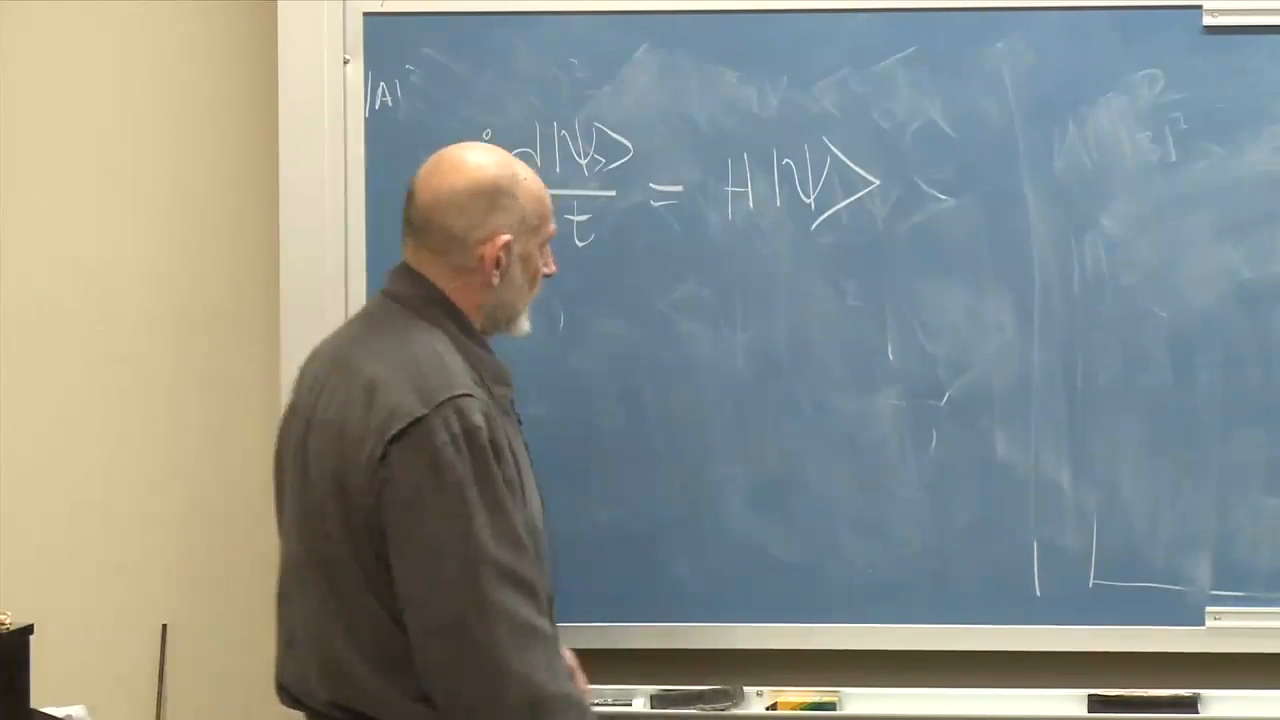
\includegraphics[width=0.88\textwidth]{lecture_10_figure_10.png}
\caption{哈密顿量作用于含时Schr\"odinger方程中的抽象态矢量。}
\lectureframe{00:59:05}
\end{figure}

在位置表象中，\(P^2\)变成二阶导数。\(X\)的函数通过乘法作用：
\begin{equation}
\bigl(V(X)\psi\bigr)(x)=V(x)\psi(x).
\end{equation}
因此，
\begin{equation}
i\hbar\frac{\partial\psi(x,t)}{\partial t}
=
\left[
-\frac{\hbar^2}{2m}\frac{\partial^2}{\partial x^2}
+V(x)
\right]\psi(x,t).
\label{eq:l10-position-schrodinger}
\end{equation}

\begin{figure}[htbp]
\centering
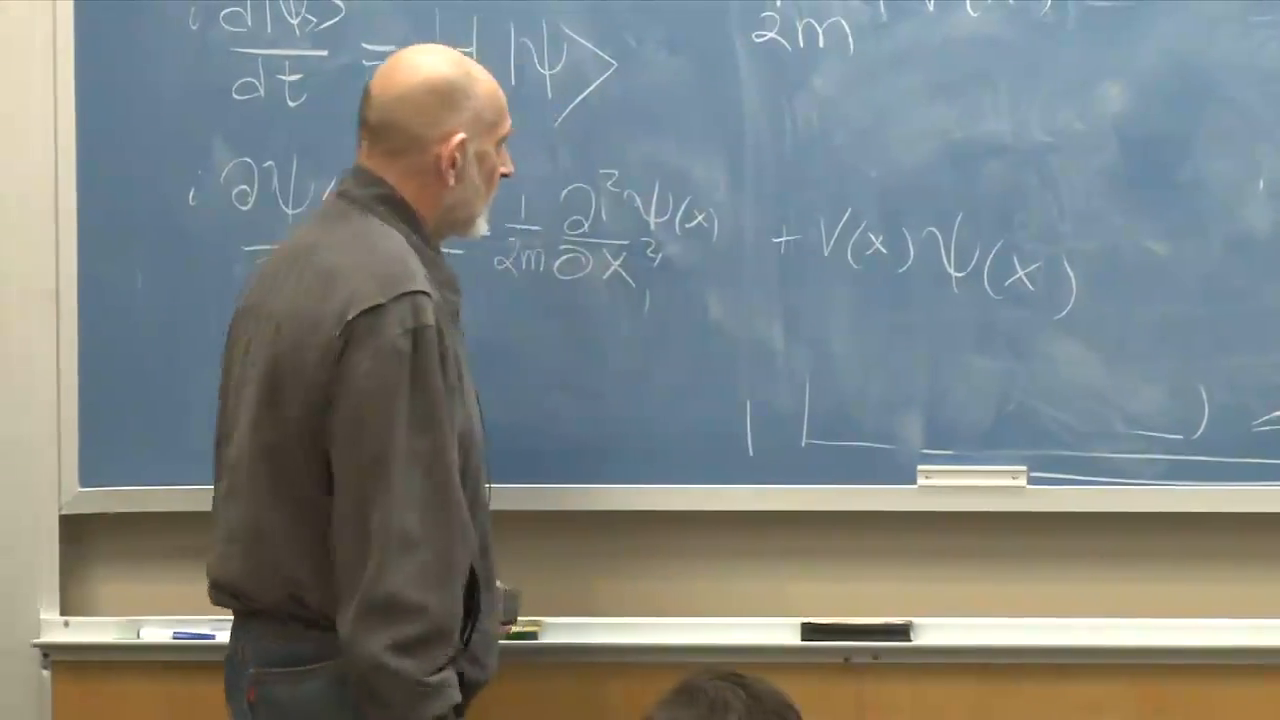
\includegraphics[width=0.88\textwidth]{lecture_10_figure_11.png}
\caption{粒子哈密顿量变成动能二阶导数加上乘以\(V(x)\)。}
\lectureframe{01:03:05}
\end{figure}

\begin{classroomqa}
\audiencequestion{普通函数\(V(x)\)在什么意义上是算子？}
\lecturerresponse{一旦选定了位置基，\(X\)就通过乘以\(x\)来作用。因此，一个足够规则的函数\(V(X)\)在每一点通过乘以相应的数\(V(x)\)来作用。它的有用性由随后的动力学来检验。}
\end{classroomqa}

对于期望值的计算，从方程~\eqref{eq:l10-position-schrodinger}解出两个时间导数：
\begin{align}
\dot{\psi}
&=
\frac{i\hbar}{2m}\psi''
-\frac{i}{\hbar}V\psi,
\label{eq:l10-psi-dot}\\
\dot{\psi}^{\,*}
&=
-\frac{i\hbar}{2m}\psi^{*\,\prime\prime}
+\frac{i}{\hbar}V\psi^*.
\label{eq:l10-psi-star-dot}
\end{align}
第二行只是第一行的复共轭，但把两者都写出来能使相消变得明显。

\section{波包中心的运动}

位置分布的中心是
\begin{equation}
\expect{X}
=
\int_{-\infty}^{\infty}
dx\,\psi^*(x,t)\,x\,\psi(x,t).
\end{equation}
对它求导：
\begin{equation}
\frac{d}{dt}\expect{X}
=
\int dx\,
\left(
\dot{\psi}^{\,*}x\psi
+
\psi^*x\dot{\psi}
\right).
\label{eq:l10-x-expectation-derivative}
\end{equation}
这两项互为复共轭。代入方程~\eqref{eq:l10-psi-dot}和\eqref{eq:l10-psi-star-dot}后，势能项相消，因为\(V(x)\)是实的。对动能项分部积分后剩下
\begin{align}
\frac{d}{dt}\expect{X}
&=
\frac{1}{m}
\int dx\,
\psi^*
\left(-i\hbar\frac{\partial}{\partial x}\right)
\psi \notag\\
&=
\frac{\expect{P}}{m}.
\label{eq:l10-ehrenfest-x}
\end{align}

\begin{figure}[htbp]
\centering
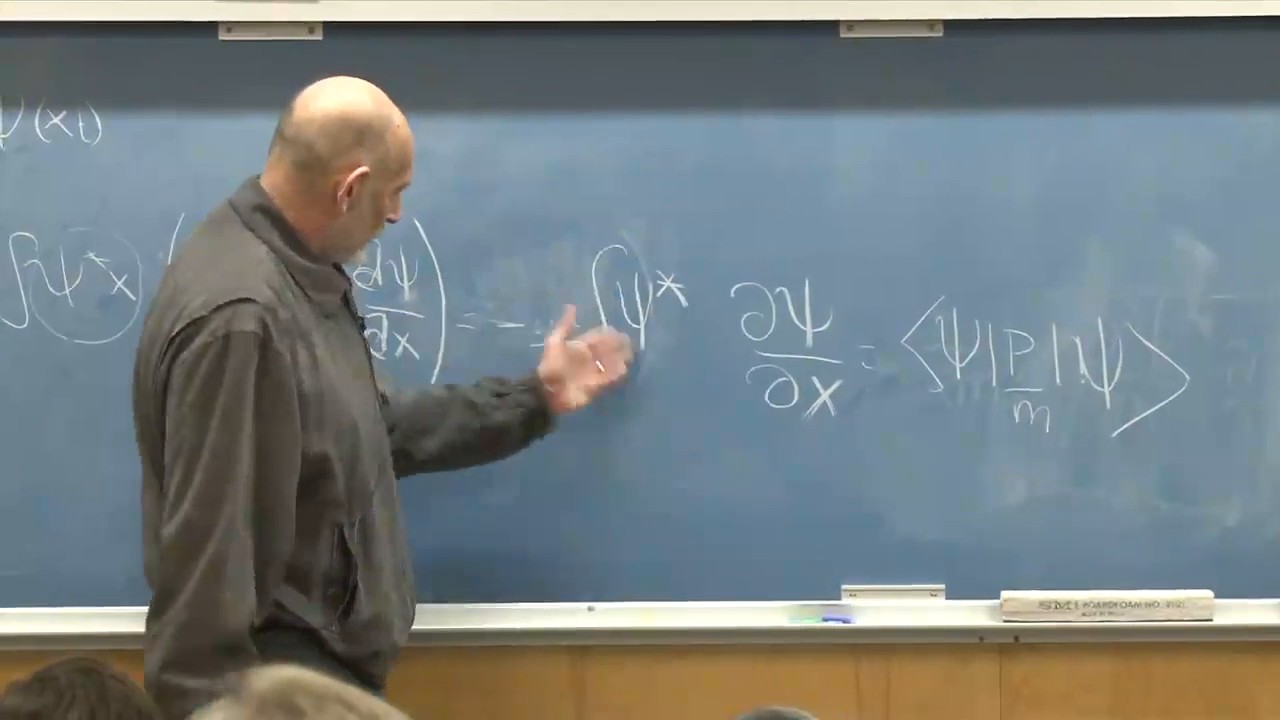
\includegraphics[width=0.88\textwidth]{lecture_10_figure_12.png}
\caption{波包中心的导数化为动量期望值除以质量。}
\lectureframe{01:15:40}
\end{figure}

这个关系是精确的。代数推导中没有引入任何窄波包近似。

\begin{classroomqa}
\audiencequestion{在这个推导中，波包是单个窄凸起这一假设用在了哪里？}
\lecturerresponse{哪里都没用。恒等式\(d\expect{X}/dt=\expect{P}/m\)对此哈密顿量定义域内的每一个态都成立。只有当我们把\(\expect{X}\)解释为经典粒子的轨迹时，局域性才起作用。}
\end{classroomqa}

力学的另一半涉及动量：
\begin{equation}
\expect{P}
=
\int dx\,
\psi^*
\left(-i\hbar\frac{\partial}{\partial x}\right)
\psi.
\end{equation}
对两个依赖于时间的因子求导：
\begin{equation}
\frac{d}{dt}\expect{P}
=
-i\hbar
\int dx\,
\left(
\dot{\psi}^{\,*}\psi'
+
\psi^*\frac{\partial\dot{\psi}}{\partial x}
\right).
\label{eq:l10-p-expectation-start}
\end{equation}
对其中一项分部积分后，代入两个Schr\"odinger方程。动能贡献相消。势能项合并为
\begin{equation}
\int dx\,
V(x)
\left(
\psi\frac{\partial\psi^*}{\partial x}
+
\psi^*\frac{\partial\psi}{\partial x}
\right)
=
\int dx\,
V(x)\frac{\partial}{\partial x}|\psi|^2.
\end{equation}
最后一次分部积分把导数移到势能上：
\begin{align}
\frac{d}{dt}\expect{P}
&=
-\int dx\,|\psi(x,t)|^2\frac{dV}{dx} \notag\\
&=
-\expect{V'(X)}
\\
&=
\expect{F(X)},\\
F(x)&=-V'(x).
\label{eq:l10-ehrenfest-p}
\end{align}

\begin{figure}[htbp]
\centering
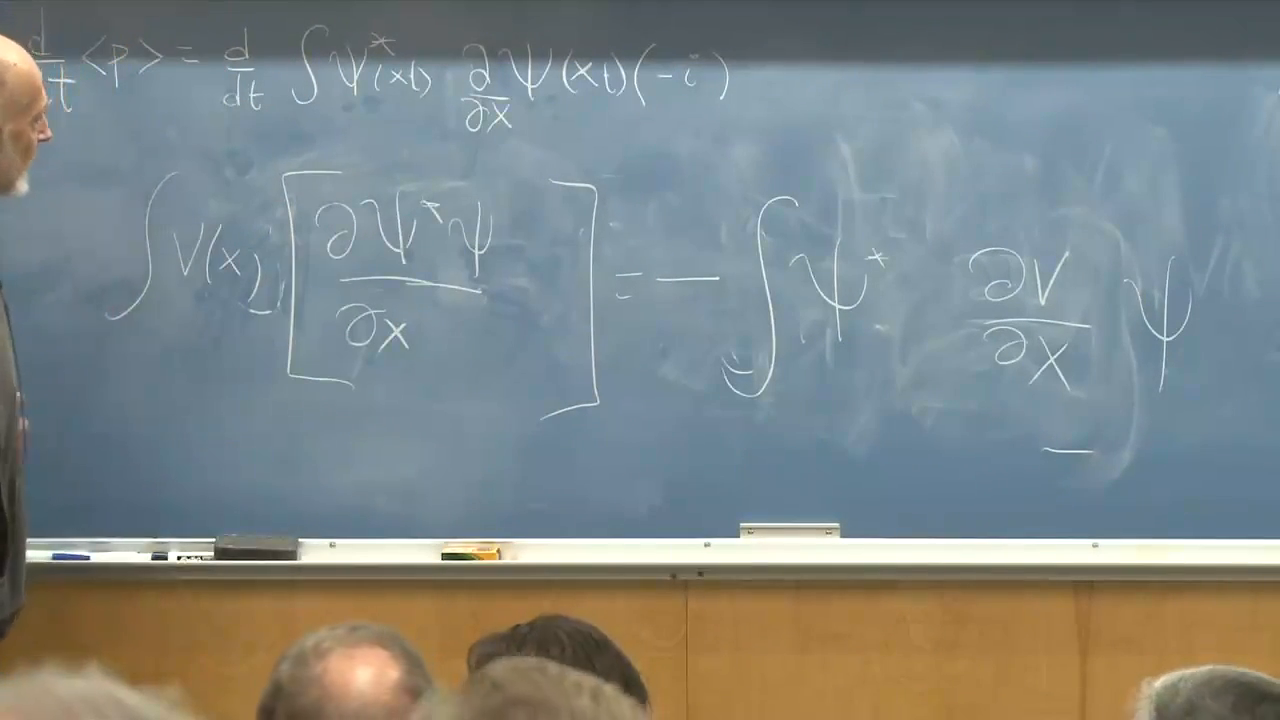
\includegraphics[width=0.88\textwidth]{lecture_10_figure_13.png}
\caption{势能项合并为一个全导数，给出\(d\expect{P}/dt=-\expect{V'(X)}\)。}
\lectureframe{01:30:45}
\end{figure}

方程~\eqref{eq:l10-ehrenfest-x}和\eqref{eq:l10-ehrenfest-p}是此哈密顿量的埃伦费斯特定理。它们是精确的量子恒等式，但精确的期望值方程还不等同于经典轨道。

\section{经典近似在哪里进入}

对于位于波包中心的点，经典力学将要求
\begin{equation}
\frac{d}{dt}\expect{P}
\approx
F\!\left(\expect{X}\right).
\label{eq:l10-classical-center-force}
\end{equation}
而量子力学给出的是
\begin{equation}
\frac{d}{dt}\expect{P}
=
\expect{F(X)}.
\end{equation}
一般而言，
\begin{equation}
\expect{F(X)}
\neq
F\!\left(\expect{X}\right).
\label{eq:l10-force-nonlinearity}
\end{equation}

\begin{classroomqa}
\audiencequestion{如果两个埃伦费斯特方程都是精确的，为什么它们还不能证明每个量子态都遵循牛顿定律？}
\lecturerresponse{波包中心的牛顿定律需要在中心处计算力。精确的量子方程包含力在整个概率分布上的平均值。对于缓慢变化的力场中的窄波包，两者一致，但对于任意态或非线性力则不然。}
\end{classroomqa}

讲座中的反例使这一区别变得无可置疑。令\(F(x)=x^2\)，并选择一个归一化态，它由两个等高的窄凸起组成，分别中心在\(+a\)和\(-a\)附近。对称性给出
\begin{equation}
\expect{X}=0,
\qquad
F\!\left(\expect{X}\right)=0,
\end{equation}
而
\begin{equation}
\expect{F(X)}
=
\expect{X^2}
\approx
a^2>0.
\end{equation}

\begin{figure}[htbp]
\centering
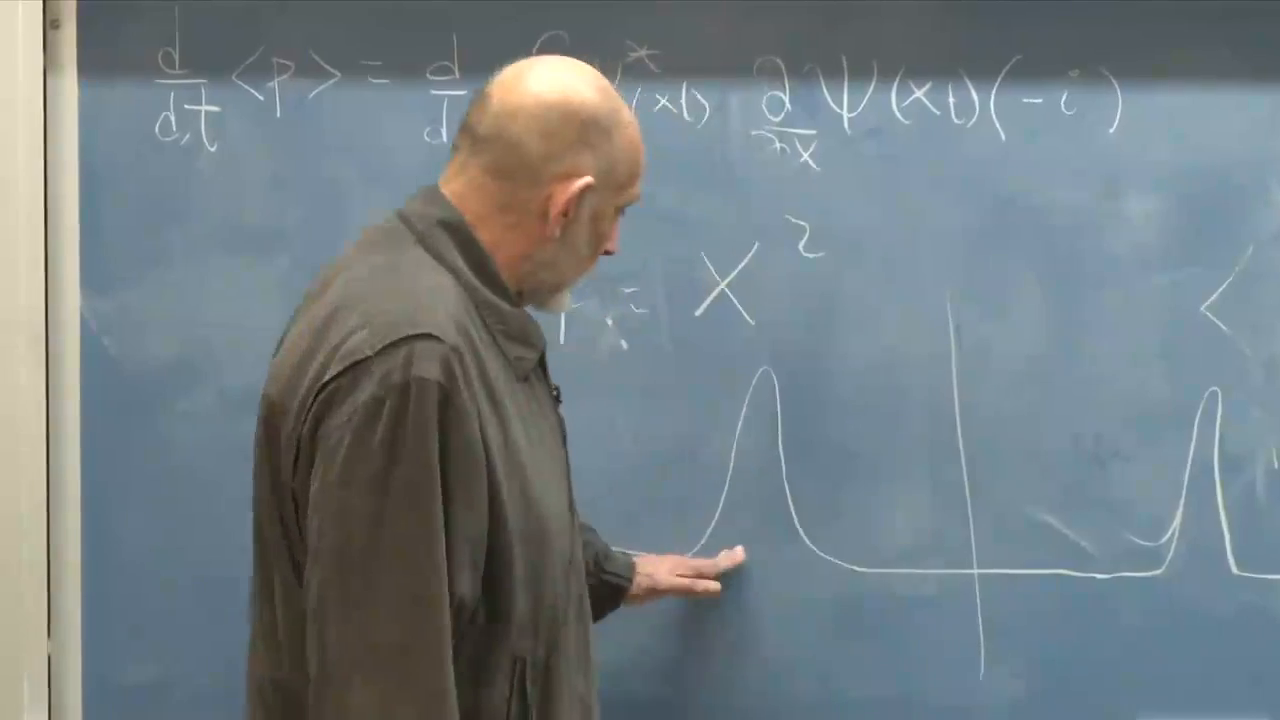
\includegraphics[width=0.88\textwidth]{lecture_10_figure_14.png}
\caption{对于对称的双凸起波包和\(F(x)=x^2\)，均值处的力为零，而力的均值不为零。}
\lectureframe{01:33:35}
\end{figure}

对于中心在\(\bar{x}=\expect{X}\)的单个窄波包，展开力：
\begin{equation}
F(X)
=
F(\bar{x})
+
F'(\bar{x})(X-\bar{x})
+
\frac{1}{2}F''(\bar{x})(X-\bar{x})^2
+\cdots.
\end{equation}
取期望值消去线性项：
\begin{equation}
\expect{F(X)}
=
F(\bar{x})
+
\frac{1}{2}F''(\bar{x})(\Delta x)^2
+\cdots.
\end{equation}
当波包与力发生显著变化的长度尺度相比仍然很窄时，经典近似是可靠的。

尖锐的特征会使波包分裂并散射。宽广而平滑的势倾向于引导一个足够局域化的波包，而不破坏其单凸起形式；点状障碍物、原子核或与波长同尺度的结构则会产生反射和衍射分量。

\begin{figure}[htbp]
\centering
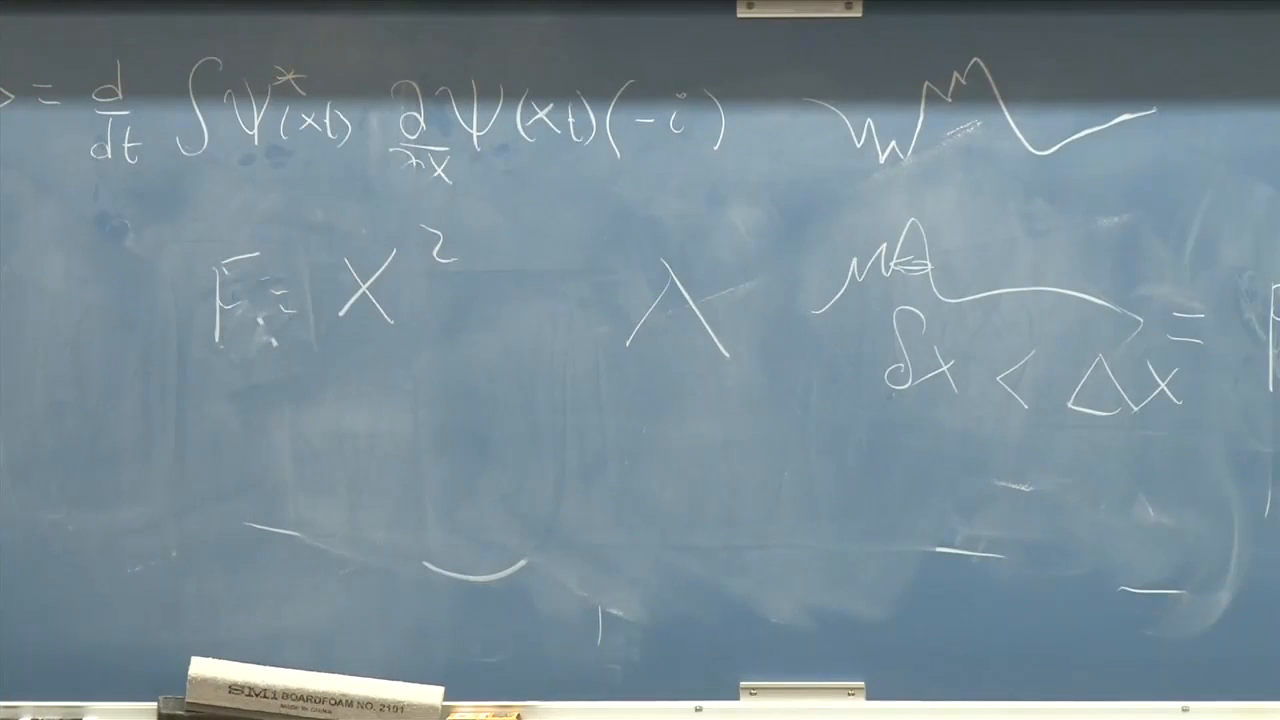
\includegraphics[width=0.88\textwidth]{lecture_10_figure_15.png}
\caption{尺度短于波包宽度或相关波长的势结构会把一个相干波包分解为散射分量。}
\lectureframe{01:37:25}
\end{figure}

\begin{classroomqa}
\audiencequestion{是什么使一个势对经典波包而言是坏的？}
\lecturerresponse{问题在于尺度，而不在于道德品质。比波包尖锐得多的特征，或与其波长相当的特征，会显现出波动本性并产生散射。如果势在波包范围内变化缓慢，则力在其支撑上几乎为常数，中心便遵循经典方程。}
\end{classroomqa}

质量也很重要。对于接近最小不确定度的波包，
\begin{equation}
\Delta x\,\Delta v
\sim
\frac{\hbar}{2m}.
\end{equation}
大质量允许既有小的空间宽度又有适中的速度展宽。因此，重物体在穿越宏观势时仍能保持高度局域化。轻粒子更容易被微观结构展宽或衍射。这是一个标度论证，而不是声称仅由质量决定运动是否为经典。

\begin{classroomqa}
\audiencequestion{在这个意义上，电子是否曾经大到足以近似地表现为经典行为？}
\lecturerresponse{是的，如果外场在电子波包的尺度上平滑变化。例如，在宽大的电容器极板之间，一个相干波包可以在一段有用的时间内遵循经典加速度。在原子核尖锐的库仑结构附近，同一个电子则表现出显著的散射。}
\end{classroomqa}

卢瑟福的1911年散射实验提供了互补的教训。{\proseunicodefont α}粒子遇到金原子核紧凑的电荷分布时被散射到大角度，揭示出正电荷集中在一个非常小的区域内。卢瑟福描述的是一束粒子；量子力学描述的是入射振幅及其散射分量。现代电子和光子散射实验利用的是同样的尺度敏感性。

\begin{classroomqa}
\audiencequestion{这种波与尺度的行为是物质粒子所特有的吗？}
\lecturerresponse{不是。当折射率在一个波长范围内缓慢变化时，电磁波遵循几何光学。间距与波长相当的衍射光栅将波展布到不同的方向上。电子、{\proseunicodefont α}粒子、光子以及其他量子激发都共享这种波长与结构之间的关系。}
\end{classroomqa}

因此，经典极限并不是粘贴在量子力学之上的另一条独立定律。精确的期望值方程已经包含了经典关系。当态保持局域化，并且哈密顿量变化足够平滑，以至于对力求平均实际上等同于在波包中心求值时，经典轨迹便会出现。
